%---------------------------------------------------------------------------
% Knowledge component.
%
%---------------------------------------------------------------------------
\section{Knowledge component}
\label{sec:arch_knowledge}

Knowledge component is responsible for realization of semantic-based approach to the proposed system. Although end-user can barely notice its existence, it is crucial to allow high scalability and ease of use. The ontologies provided by the system provides generic measurement semantics. Such an approach allows the user to get to know the system only once and work using it with many different types of hardware, protocols. He or She can work with any measurable item types that can be mapped into generic components introduced by ontologies. Additionally it allows to work with all those different items simultaneously; thus, it makes it possible to monitor an application that is written using different, cooperating technologies.

\subsection{Default ontologies}

All system functionalities are built around two main ontologies - the first one grouping resources, and the second, covering resource capabilities. The main principle, I was trying to follow when designing them was to maximize the range of applications that can be monitored using the SemSimMon system - from those running single process on one computing machine, up to highly distributed, grid-oriented ones.

Two root concepts must be explained: the concept of resource and of capability, in order to describe the proposed ontologies in more detail. The resource class wraps all components that are used to perform required computations. Resource can be a physical device that takes part in computation (hardware resources), or any software component that is either a dependency (library) or one that the user creates (program, library). The capability concept generalizes all measurable features of each resource. Capabilities exist only in the context of resources that contain them. Resource may have multiple capabilities and a given capability may exist within the context of multiple resources.

Both these ontologies are described using diagrams containing two types of relationships: \lq\lq{}\emph{is-a}\rq\rq{}, and \lq\lq{}\emph{has-a}\rq\rq{}. Is-a relationship, is formalized as \texttt{rdfs:subClassOf} and states that all instances of one class are instances of another~\cite{rdfRef:2004}. The \lq\lq{}\emph{has-a}\rq\rq{} relationship describes resources only. The main purpose of this relationship is to show composition arrangement. It aims at easing understanding of which resources a given parent resource use (e.g. virtual machine uses class loader, garbage collector; one or more CPUs builds computing node, storage device, network device, and so on).

In the diagrams that follow, entities are drawn as a filled ellipse with an entity name inside. The graphical representation of the \lq\lq{}\emph{is-a}\rq\rq{} relationship between two entities is a hollow triangle shape on the super type end of the line that connects it to one or more subtypes. Diagrams use a line with an arrowhead indicating an owned side of a relationship to represent \lq\lq{}\emph{has-a}\rq\rq{} relation. UML use case diagram specification was the source of inspiration for this notation.

\subsection{Resources ontology}
\label{subsec:arch_knowledge_resources}

Complexity of the resources ontology , forced me to split diagrams containing both \lq\lq{}\emph{is-a}\rq\rq{} and \lq\lq{}\emph{has-a}\rq\rq{} relationships into 3 parts: the one containing most general classes (application, node, and cluster), the second one for hardware resources and the third one, covering the software resources. 

\begin{figure}[ht]
\centering
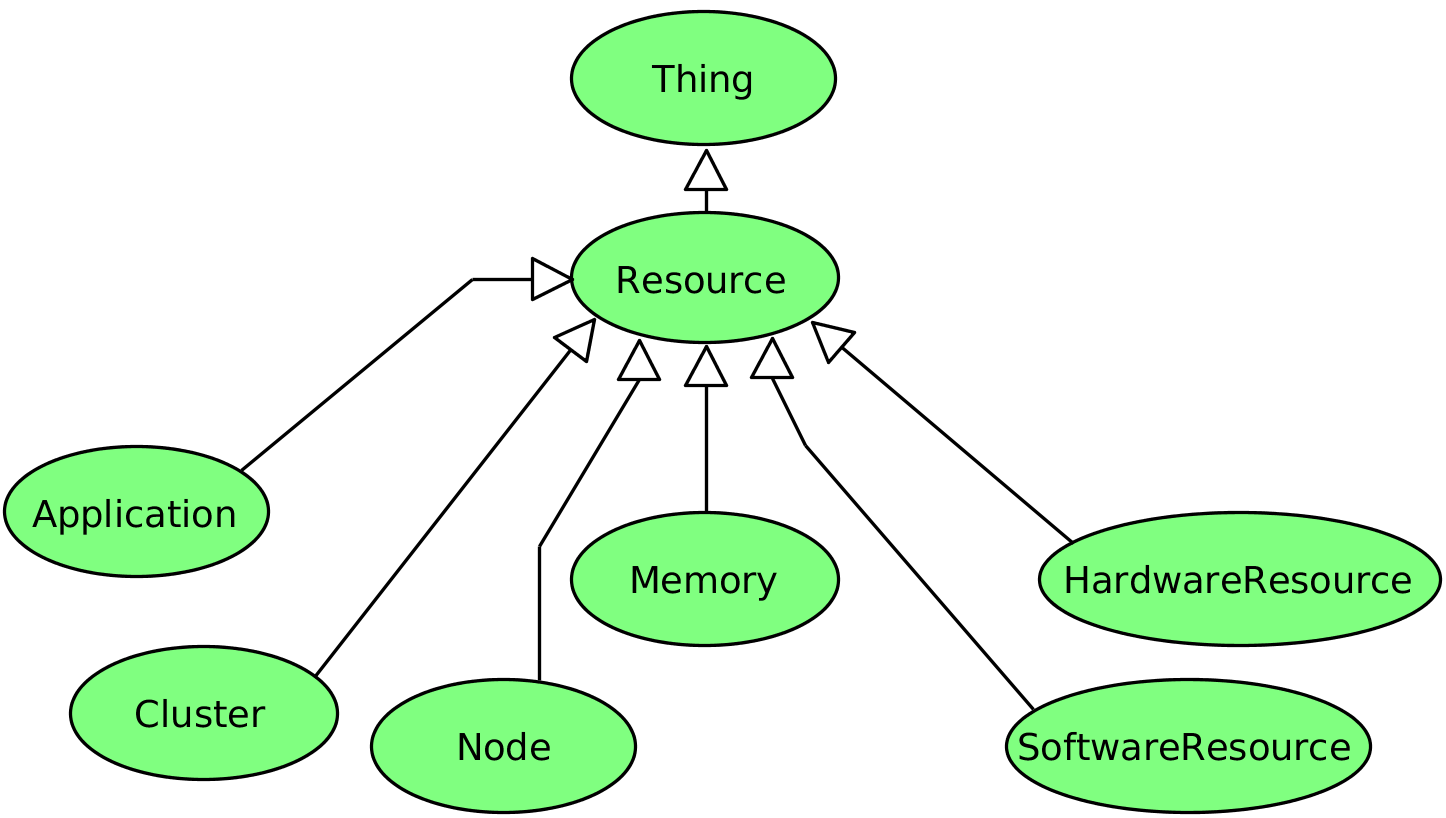
\includegraphics[width=0.6\textwidth]{onto_resources_admin}
\caption{Diagram of the \lq\lq{}\emph{is-a}\rq\rq{} (rdfs:subClassOf) relationship between most general resource concepts}
\label{fig:onto_resources_admin}
\end{figure}

Figure~\ref{fig:onto_resources_admin} depicts i\lq\lq{}\emph{is-a}\rq\rq{}a relationship between general SemSimMon\rq{}s concepts. The root class of each entity in OWL compliant ontologies is \texttt{owl:Thing}, as specified in OWL language reference~\cite{owlRef:2009}. I have introduced a generic \texttt{Resource} class to cover all possible resources. It acts as a root concept for all other resources and the only one that is a direct subclass of \texttt{owl:Thing}. \texttt{Resource} has 6 direct subtypes: \texttt{Application}, \texttt{Cluster}, \texttt{Node}, \texttt{Memory}, \texttt{HardwareResource} and \texttt{SoftwareResource}. \texttt{Application} and \texttt{Cluster} types are so called \lq\lq{}management\rq\rq{} class resources - they do not represent actual components, which can be used to perform computations. Instead, they can be used to aggregate one or more elements, which allows the user to build more manageable measurement structures. \texttt{Application} is the most notable entity type, in the context of the \lq\lq{}\emph{has-a}\rq\rq{} relationship, which is illustrated in Figure~\ref{fig:onto_resources_has_a_admin}. It represents a program created by the user that he or she wants to analyze using the proposed tool. Each application, in a a theoretical model may be running on multiple clusters, and multiple nodes.

\texttt{Cluster} refers to a group of computing nodes, which are connected using a high-efficiency network; thus, in some way may be treated as a single entity. It is equivalent of \lq\lq{}site\rq\rq{} in the OMIS nomenclature~\cite{tl9702e}. A \texttt{Node} can be interpreted as a bridge between high-level resources and software, hardware resources. It is the smallest independent computing unit, e.g. a single PC or a unit in a rack. It can be treated as an administrative resource type, as it is not a component that is used directly, but one that those components. On the other hand, a node is an actual processing device.

There exists also a noteworthy class of resources - \texttt{Memory}. It was created, because there exists at least two types of memory: software based (virtual memory) and hardware (physical memory) that share common semantics that can be easily described in this type.

\begin{figure}[ht]
\centering
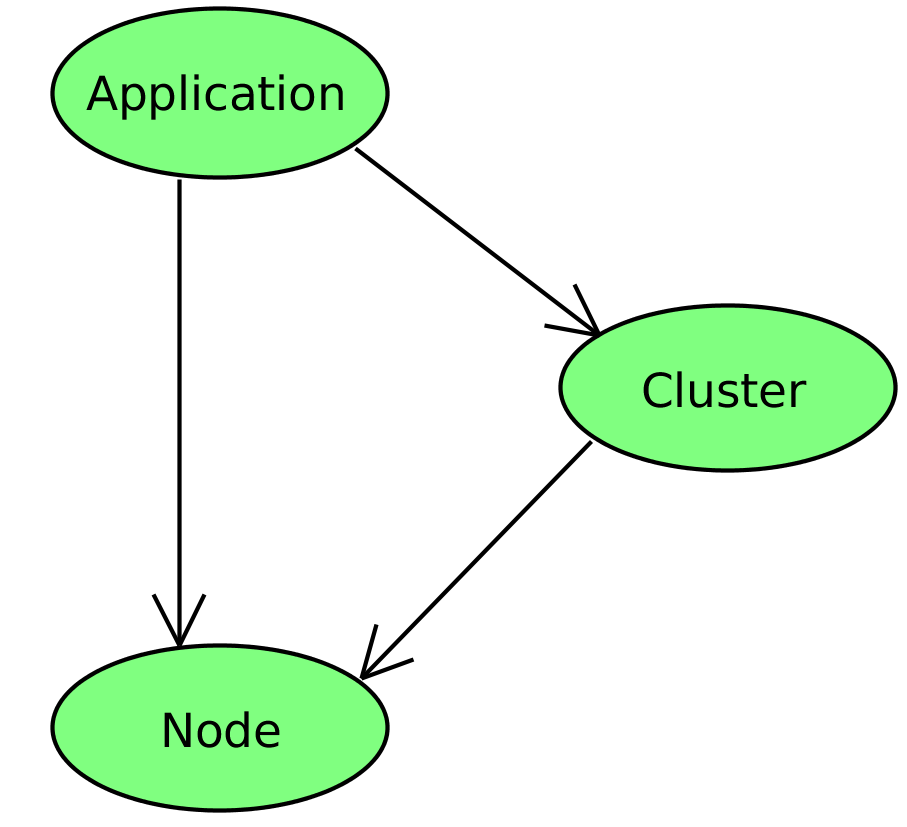
\includegraphics[width=0.3\textwidth]{onto_resources_has_a_admin}
\caption{Diagram of the \lq\lq{}\emph{has-a}\rq\rq{} relationship between most general resource concepts}
\label{fig:onto_resources_has_a_admin}
\end{figure}

\begin{figure}[ht]
\centering
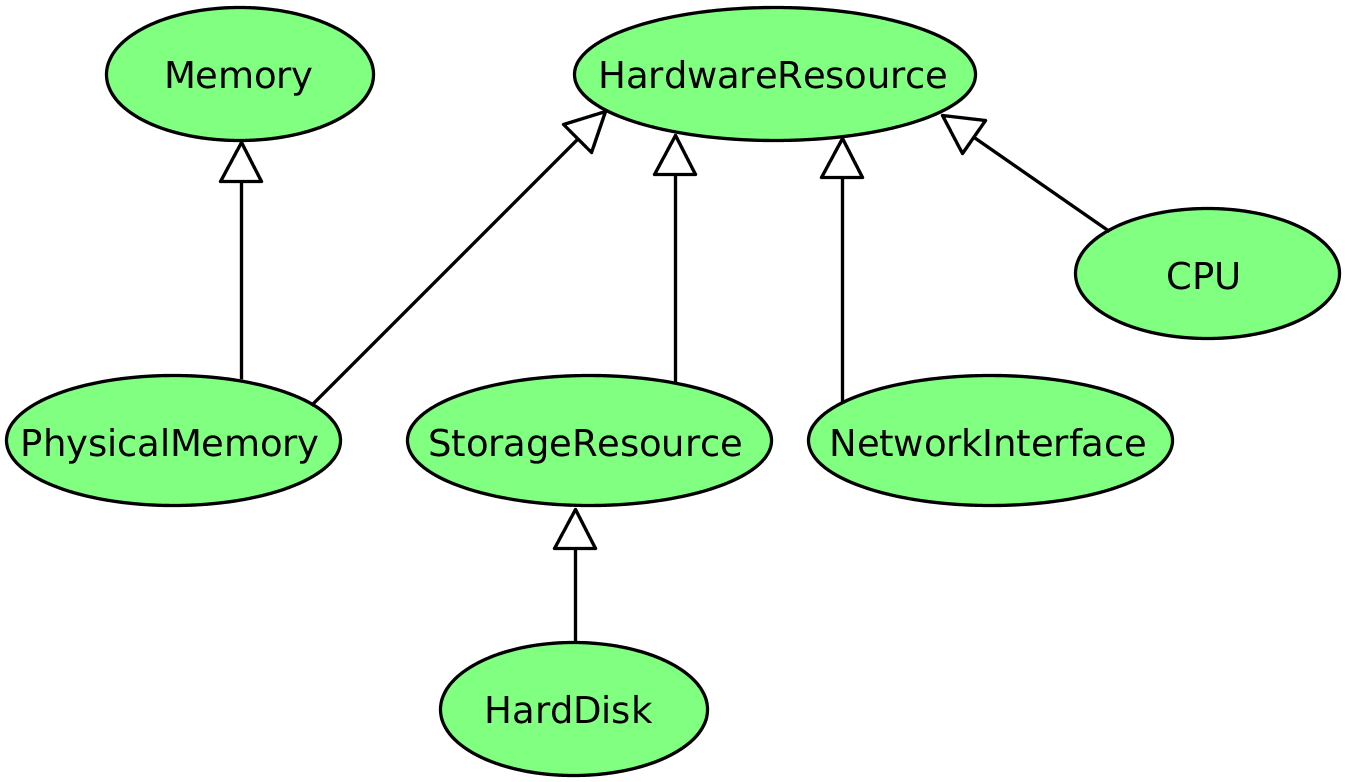
\includegraphics[width=0.6\textwidth]{onto_resources_hardware}
\caption{Diagram of \lq\lq{}\emph{is-a}\rq\rq{} relationship between hardware resources}
\label{fig:onto_resources_hardware}
\end{figure}

The classes related to hardware resources, can be seen in Figures~\ref{fig:onto_resources_hardware} and~\ref{fig:onto_resources_has_a_hardware}. The design of all of them allows covering most of computer parts available nowadays on the market. Both diagrams are quite straightforward. \texttt{HardwareResource} has 4 direct sub-types: \texttt{PhysicalMemory}, \texttt{StorageResource}, \texttt{NetworkInterface} and \texttt{CPU}. \texttt{PhysicalMemory}, is also a subtype of the \texttt{Memory} class, to share common semantics. Also, \texttt{StorageResource} has one derived class - \texttt{HardDisk}. Hardware resources\rq{} \lq\lq{}\emph{has-a}\rq\rq{} relationship diagram is even more elementary - \texttt{Node} may have all hardware resources, and there are no other relations between those resources.

\begin{figure}[ht]
\centering
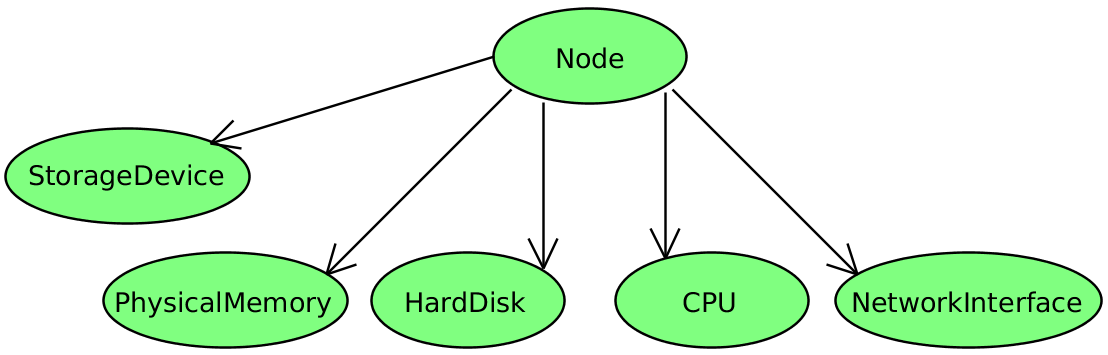
\includegraphics[width=0.7\textwidth]{onto_resources_has_a_hardware}
\caption{Diagram of \lq\lq{}\emph{has-a}\rq\rq{} relationship between hardware resources}
\label{fig:onto_resources_has_a_hardware}
\end{figure}

\begin{figure}[ht]
\centering
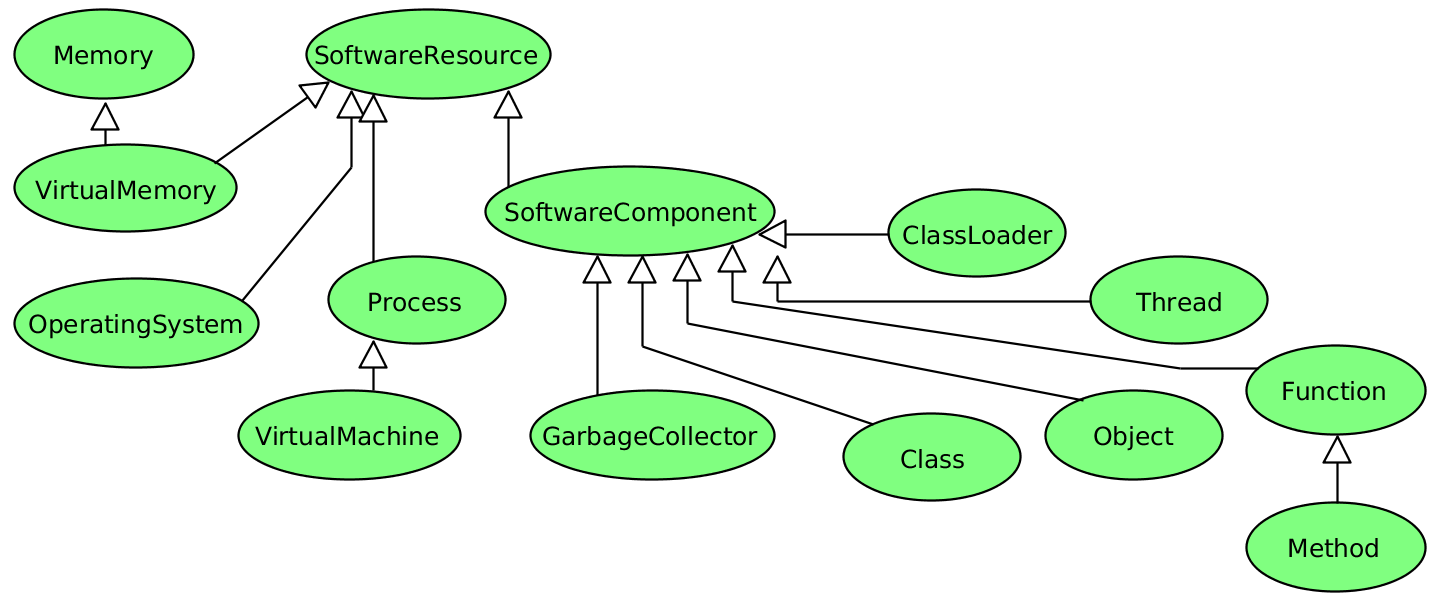
\includegraphics[width=0.9\textwidth]{onto_resources_software}
\caption{Diagram of is-a relationship between software resources}
\label{fig:onto_resources_software}
\end{figure}

The system is aware of more software then hardware resource types. This implies sophisticated relationships between concepts depicted in Figures~\ref{fig:onto_resources_software} and~\ref{fig:onto_resources_has_a_software}. Class \texttt{SoftwareResource} has 4 direct subtypes: \texttt{VirtualMemory} (which also derives from the generic \texttt{Memory} concept), \texttt{OperatingSystem}, \texttt{Process} and \texttt{SoftwareComponent} concept. First three types are quite straightforward and represent what one expects them to do. A special subtype of \texttt{Process}, namely \texttt{VirtualMachine} needs more concern. It was extracted from a general type, because of its nature, which differs it from all general-purpose processes. Each virtual machine acts as a runtime environment for running applications; thus, it has features common for all virtual machines, but unlikely seen in casual process. The \texttt{SoftwareComponent} resource type is a logical wrapper for all low level software components that can be used to create a program. There are generic components, like \texttt{Thread}, \texttt{Function}. There are also types specific to Object Oriented Programming: \texttt{Class}, \texttt{Object}, and \texttt{Method} (which subtypes \texttt{Function}). The third group of \texttt{SoftwareComponent} subtypes is specific to virtual machines. It contains only two items: \texttt{GarbageCollector} and \texttt{ClassLoader}.

Regarding ownership relations in the software category there is one root concept - \texttt{Node}. Each node has \texttt{OperatingSystem}, and multiple \texttt{Processes}. Some processes may be a \texttt{VirtualMachine}, which makes this resource is the last type that \texttt{Node} may directly own. Each \texttt{Process} may have the following software components: \texttt{Thread}, \texttt{Object}, \texttt{Class} and \texttt{Function}. \texttt{VirtualMachine} may have all components that the generic \texttt{Process} has and two more specific: \texttt{ClassLoader} and \texttt{GarbageCollector}. Additionally, \texttt{Class} type owns single one resource type, the \texttt{Method}. The \texttt{OperatingSystem} resource may have only one software resource type, namely \texttt{VirtualMemory}.

\begin{figure}[ht]
\centering
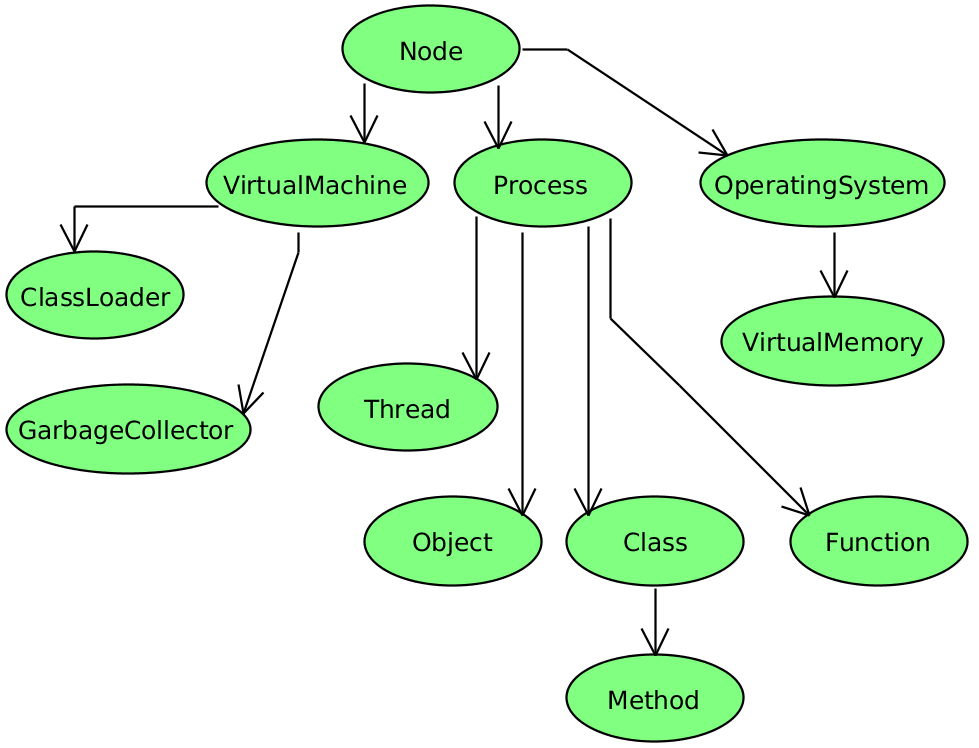
\includegraphics[width=0.7\textwidth]{onto_resources_has_a_software}
\caption{Diagram of \lq\lq{}\emph{has-a}\rq\rq{} relationship between software resources}
\label{fig:onto_resources_has_a_software}
\end{figure}

\pagebreak

\subsection{Capabilities ontology}
\label{subsec:arch_knowledge_capabilitie}

For the concepts related to the capabilities of resources, only the \lq\lq{}\emph{is-a}\rq\rq{} relationship was defined, which is illustrated in Figure~\ref{fig:onto_capabilities}. There is one root concept, namely \texttt{ResourceCapability}, which subclasses \texttt{rdf:Thing}. It has 4 direct subtypes: \texttt{HardwareCapability}, \texttt{MemoryCapability}, \texttt{NodeCapability} and \texttt{SoftwareCapability}. \texttt{HardwareCapability} has only 2 derived classes: \texttt{StorageCapability} and \texttt{CpuCapability}. Since the concepts of \texttt{VirtualMemory} and \texttt{PhysicalMemory} are semantically close, there is no need to subclass generic MemoryCapability; thus, this type does not have any subtypes. \texttt{NodeCapability} is another direct subtype of the most generic \texttt{ResourceCapability}, which does not require any additional child types.

The complex structure of software resources influences relationships between the capabilities related to those components. \texttt{SoftwareCapability} has 3 subtypes: \texttt{OperatingSystemCapability}, \texttt{ProcessCapability} and \texttt{SoftwareComponentCapability}. Additionally, \texttt{VirtualMachineCapability} was extracted from \texttt{ProcessCapability}, because of the same reasons that motivate the extraction of \texttt{VirtualMachine} resource type from \texttt{Process} - different semantics. The single type that extends \texttt{SoftwareComponentCapability} is \texttt{ThreadCapability}.

\begin{figure}[ht]
\centering
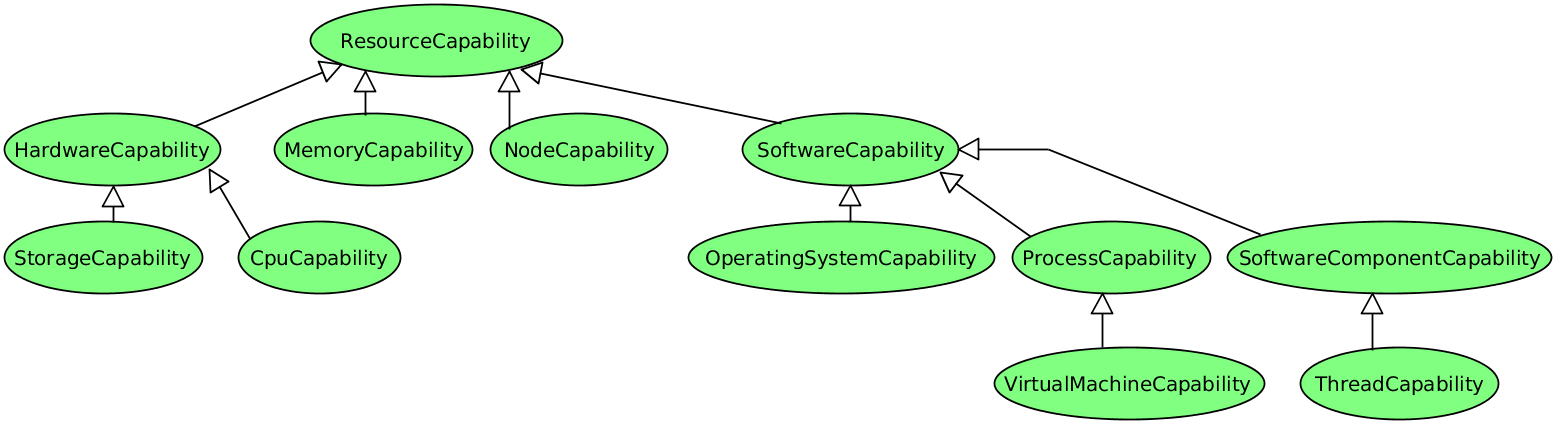
\includegraphics[width=1.0\textwidth]{onto_capabilities}
\caption{Diagram of the \lq\lq{}\emph{is-a}\rq\rq{} relationship between capabilities}
\label{fig:onto_capabilities}
\end{figure}

